% !TEX root = ./Research_and_SA.tex

% FROM THE NIH SITE:
% Is the proposed research project of high scientific quality, and is it well integrated with the proposed research training plan?
% Based on the sponsor’s description of his/her active research program, is the applicant’s proposed research project sufficiently distinct from the sponsor’s funded research for the applicant’s career stage?
% Is the research project consistent with the applicant’s stage of research development?
% Is the proposed time frame feasible to accomplish the proposed training?

\textbf{SIGNIFICANCE}\\
RNA lies at the center of cellular function. Its most appreciated function is to carry protein blueprints to the ribosome for manufacture. Only recently have researchers begun to appreciate its myriad of other functions, many of which also lie at the center of important cellular processes and disease\cite{CechNoncodingRNARevolution2014,DellaRagioneNoncodingRNAschromatin2014}.
% TODO maybe a bit more general discussion here? talk about how tracking RNA location is important generally, for all types of RNA? Then dive in to some specific examples?
Long, noncoding RNA (lncRNA) comprise one such important class of RNA that does not participate in the central dogma\cite{RinnGenomeRegulationLong2012}. Alarmingly, the human genome encodes for as many lncRNA as proteins\cite{Rinntranscriptionalactivityhuman2003}.
These biomolecules regulate localization of protein complexes within chromatin
\comment{X, Y, and Z (maybe the proposed test systems??)} have been recently found to have crucial RNA components.
\comment{Need more on these systems here. Talk about how localization is important.}
% AMY Yes you could talk about localization here.  Or you could make a figure that provides an overview of different types of RNAs and how they change localization at different points in their lifecyle.  I have a slide on this but the figure is poor quality.  I will send to you.
This importance for cellular function necessitates a toolset of probes to study these RNAs as they traverse the cell.

%%%%%%%%%%%%%%%%%%%%%%%%%%%%%%%%%%%%%%%%%%%%%%%%%%%%%%%%%%%%%%%%%%%%%%%%%%%%%%%%
%Riboglow
%\begin{wrapfigure}[30]{R}{9cm}
\begin{wrapfigure}{R}{8cm}
%\vspace{-0.2in}
\begin{centering}
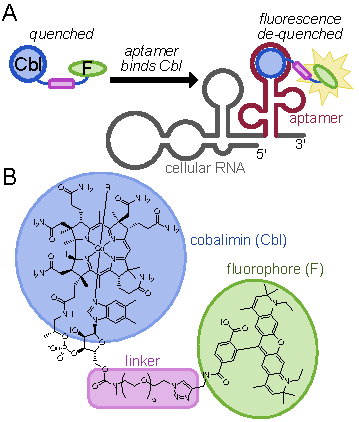
\includegraphics[width=\textwidth]{figures/fig1v2.pdf}

\end{centering}
\footnotesize
\caption{\label{figure:riboglow}
A) Cobalamin acts as a quenching and localization moiety to guide a fluorescent probe to an RNA transcript of interest. When unbound, fluorescence is quenched. In the presence of RNA tagged with the cobalamin riboswitch, fluorescence is restored. B) Structure of the generation 1 Riboglow probe. A polyethylene glycol linker of five units (5xPEG) connected to the 5' hydroxly of the cobalamin ribose was used to tether an ATTO 590 fluorophore to the construct.
}
\end{wrapfigure}
%%%%%%%%%%%%%%%%%%%%%%%%%%%%%%%%%%%%%%%%%%%%%%%%%%%%%%%%%%%%%%%%%%%%%%%%%%%%%%%%

\textbf{BACKGROUND}\\
Protein studies benefit from a large imaging toolkit that has been developed over the last 25 years. Genetically encodable fluorescent proteins are now ubiquitous for the study of the localization of any translated target in the cell. While fluorescent proteins are a mature, well-understood technology, tools for imaging the localization of individual RNA transcripts in living cells remain limited. The most popular systems to date include dye-binding aptamers (Spinach\cite{PaigeRNAMimicsGreen2011}, Broccoli\cite{FilonovBroccoliRapidSelection2014}, and Mango\cite{AutourFluorogenicRNAMango2018,DolgosheinaRNAMangoAptamerFluorophore2014}), and RNA-binding protein fusions (MS2-FPs)\cite{FuscoSinglemRNAMolecules2003}.

The most analogous to fluoresecent proteins, dye-binding aptamers utilize exogenously administered dyes that give fluorescence induction upon binding their RNA partner\cite{PaigeRNAMimicsGreen2011,FilonovBroccoliRapidSelection2014,AutourFluorogenicRNAMango2018,DolgosheinaRNAMangoAptamerFluorophore2014}.
This sequence is encoded downstream of an RNA of interest to track its location in the cell. Though excellent binders for their dyes, the aptamers utilized by this technology are unstable in mammalian cells due to their nonnative structure\cite{EtzelSyntheticRiboswitchesPlug2017}. % TODO also cite refs 37-39 from the updated Riboglow paper.
Additionally, though fluorescence turn-on is excellent \textit{in vitro}, often reaching 1,000 fold, signal induction in cells is typically two to four fold, most likely due to nonspecific binding of the dye.

RNA-binding protein fusions are a much more robust technique for imaging RNA transcripts\cite{FuscoSinglemRNAMolecules2003}. This method often utilizes the MS2 bacteriophage coat protein that binds an encoded stem loop of RNA. When MS2 is fused to a fluorescent protein, transcripts can be visualized in the cell. In order to concentrate the fluorescence signal above background, multiple stem loops are placed in series (up to 24 in a row). Though this technique has enabled imaging of single transcripts in the cell\cite{MorisakiRealtimequantificationsingle2016,FuscoSinglemRNAMolecules2003}, the resulting protein-RNA complex is prohibitively large for many studies.

Riboglow is a recently developed platform in the Palmer lab that solves many of the drawbacks of current RNA imaging techniques (Fig. \ref{figure:riboglow})\cite{BraselmannDevelopmentriboswitchbasedplatform2017}. The two-component system utilizes a synthetic fluorophore-quencher pair, and a genetically-encoded riboswitch. A transcript of interest is first tagged within the cell, and the probe construct is administered via bead loading\cite{McNeilGlassbeadsload1987,Hayashi-TakanakaTrackingepigenetichistone2011,MorisakiRealtimequantificationsingle2016}.
When the construct binds the transcribed riboswitch, the fluorophore is dequenched, giving fluorescent signal. Like the dye-binding aptamers, Riboglow utilizes a riboswitch receptor domain that natively binds vitamin B\textsubscript{12} (cobalamin, Cbl, Fig. \ref{figure:riboglow}B)\cite{JohnsonJrB12cofactorsdirectly2012}.
Conveniently, cobalamin is known to act as a fluorescence quencher for a variety of fluorophores\cite{RosendahlSynthesisbiologicalactivity1982,LeeDesignSynthesisCharacterization2009,SmeltzerSynthesisCharacterizationFluorescent2001}.
The cobalamin center is conjugated to the fluorophore through a flexible linker that promotes quenching in the unbound state, but enables the fluorophore to reside at a distance in the bound state (Fig. \ref{figure:riboglow}B).

The Palmer lab found that this initial generation of Riboglow has the potential to outperform the existing tools in the field. Its use of a naturally occurring riboswitch imparts stability to the construct that is not present in aptamer-based techniques. Additionally, the use of a donor-quencher pair reduces nonspecific fluorescence in the unbound state. Such signal induction is low in the aptamer-binding dyes, and cannot be obtained at all with the MS2-fluorescent protein fusions. Due to these advantages, Riboglow outperformed Broccoli and the MS2 system in initial studies of stress granule (SG) detection in mammalian cells.

Though promising, the initial iteration of Riboglow has significant room for improvement. With initial constructs, signal induction upon riboswitch binding never exceeded seven fold \textit{in vitro}, and the pendant dye was never fully quenched (with 10-20\% residual fluorescence). Additionally, to effectively detect stress granules, four riboswitches had to be placed in series to concentrate fluorescence signal. This high background precluded single-molecule imaging. Finally, the strategy cannot currently be used to monitor the location of multiple transcripts in tandem. Herein, I will propose strategies to overcome these limitations through simultaneous modulation of the small molecule construct and riboswitch sequence. This is an undertaking for which I am uniquely suited, due to my experience of tandem modification of small molecule-protein interactions during my graduate studies. First, I will synthesize a variety of new Riboglow probes to optimize fluorescence quenching (Aim 1). Next, I will turn to the sequence of the riboswitch itself. I'll design a screen for brightness that will select the best riboswitch sequence to match the optimized probe structure (Aim 2). This new, brighter pair will be tested for single-molecule detection. Finally, I will use SELEX to identify mutually orthogonal probe-riboswitch pairs for multicomponent RNA imaging (Aim 3).

\textbf{APPROACH \underline{Aim 1.} Synthesize improved Riboglow probes.}\\
%%%%%%%%%%%%%%%%%%%%%%%%%%%%%%%%%%%%%%%%%%%%%%%%%%%%%%%%%%%%%%%%%%%%%%%%%%%%%%%%
%Aim 1
%\begin{wrapfigure}[25]{l}{10cm}
\begin{wrapfigure}{r}{12cm}
%\vspace{-0.2in}
\begin{centering}
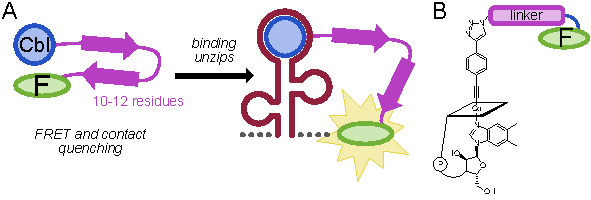
\includegraphics[width=\textwidth]{figures/aim1v3.pdf}

\end{centering}
\footnotesize
\caption{\label{figure:aim1}
A) Tryptophan zipper peptides will be used to maximize FRET and contact quenching in the unbound state. B) Conjugation via the axial site of the cobalt metal center will provide additional probe structural diversity.
}
\end{wrapfigure}
%%%%%%%%%%%%%%%%%%%%%%%%%%%%%%%%%%%%%%%%%%%%%%%%%%%%%%%%%%%%%%%%%%%%%%%%%%%%%%%%
The main drawback of Riboglow is the poor turn-on that is observed upon probe binding. In this aim, I intend to leverage my background in synthetic chemistry to produce a panel of diverse probe structures that improve fluorescence quenching (and thus signal induction). In previous studies in collaboration with Professor Dorota Gryko (see Gryko letter of support) a small number of linkers and fluorophores were evaluated for quenching and fluorescence turn-on. Linker length and fluorophore wavelength were varied to gauge the quenching ability of cobalamin. Remarkably, some degree of quenching occurred in all of the constructs synthesized, regardless of the spectral overlap of the fluorophore and the cobalamin. However, most retained 10-20\% residual fluorescence, which increased background signal significantly. \textit{To optimize probe function, I will vary linker composition, attachment point, and pendant fluorophore.}

\begin{wraptable}{L}{10cm}
\caption{Tryptophan zippers of varying stability will be tested to maximize fluorescence quenching. Values were obtained from Ref. \cite{FesinmeyerEnhancedHairpinStability2004}.}\label{linkers}
\begin{tabular}{c | c >{\centering\arraybackslash}m{1.5cm} } % funky greater than thing centers wrapped text in the cell
\toprule
Sequence & Tm ($^\circ$C) &  \% folded (25 $^\circ$C) \\\toprule
KKWTW-NPATGK-WTWQE & 85 & >96 \\
KKYTW-NPATGK-WTVQE & 66 & 92 \\
GEWTY-NPATGK-FTVTE & 47 & 74 \\  \hline
GGGGG-GGGGGG-GGGGG & N/A & N/A \\
\bottomrule
\end{tabular}
\end{wraptable}

Ideally, in the unbound state, the cobalamin and fluorophore would be closely associated to maximize FRET and contact quenching\cite{RosendahlSynthesisbiologicalactivity1982,ShellVitaminB12Tunable2015,ShellTunableVisibleNearIR2014}.
In the RNA-bound state, the molecules would reside at their maximal distance to promote fluorescence\cite{LeeDesignSynthesisCharacterization2009}.
To strike this balance, I will use a synthetic beta turn as the linker between cobalamin and the fluorophore (Fig. \ref{figure:aim1}A, Table \ref{linkers}).
Such a linker would hold the molecules close in solution, but would be linearized upon binding to the riboswitch.
A number of such beta turns have been developed, and are referred to as tryptophan zippers (trpzip)\cite{CochranTryptophanzippersStable2001}.
These motifs are as small as twelve amino acids and many are stable to denaturation up to 85 $^\circ$C (Table \ref{linkers}).
In the unbound state, such a linker would hold the quencher and fluorophore in close proximity (due to the short distance between the N and C termini of the peptide, Fig. \ref{figure:aim1}A).
When the cobalamin is bound by the riboswitch, steric occlusion would force the beta turn to unfold to place the fluorophore-quencher pair at a larger distance.
A wide range of tryptophan zippers have been developed with a varitey of structures and stabilities, enabling easy synthesis of a range of different linkers via solid phase peptide synthesis\cite{CochranTryptophanzippersStable2001,KierProbingLowerSize2008,AndersenMinimizationOptimizationDesigned2006,FesinmeyerEnhancedHairpinStability2004}.
Cobalamin and a fluorophore will then be coupled to each terminus of the linker via additional amide couplings\cite{JackowskaVitaminB12derivatives2018}.
A starting set if linkers are listed in Table \ref{linkers}.
The polyglycine linker will be used as a negative control for a linker with little secondary structure, but identical length.
If the fold proves to be too stable (dequenching is not observed), the amino acids of the peptide linker will be varied to tune the melting temperature.
Or, if adequate quenching is not observed, the relative positions of the N and C termini will be adjusted based upon structural data available on these beta turns, available in the Protein Data Bank (PDB).
Each new construct will be tested for their ability to quench fluorescence in vitro by comparing the fluorescence of the construct with that of the free fluorophore in solution. Fluorescence signal in the presence of the Riboglow riboswitch will also be measured to calculate fluorescence turn-on.

Another underexplored variable of the original Riboglow probes is the linker attachment point.
Though the 5' hydroxyl of the cobalamin ribose is the most accessible nucleophile on the structure, there exist several other possible sites of conjugation.
Perhaps the second most common site is the axial ligand of the cobalt metal itself.
Though many studies have taken advantage of the labile nature of certain alkyl modifications at this position\cite{ShellVitaminB12Tunable2015}, others have found alkynyl modifications to be stable to air and light\cite{ChrominskiReductionfreesynthesisstable2013,RuetzMarkusPhenylethynylcobalaminLightStable2013}.
Following this precedent, I will synthesize a cobalamin with an alkyne handle attached to the cobalt metal center (Fig. \ref{figure:aim1}B).
Such a molecule has already been synthesized in the lab of Dorota Gryko (see Gryko letter of support), and shown to be amenable to functionalization via dipolar azide-alkyne cycloaddition (AAC)\cite{ChrominskiVitaminB12Derivatives2014}.
The alkyne handle will be readily conjugated to a variety of linkers with terminal azides\cite{KolbHartmuthC.ClickChemistryDiverse2001,PattersonFindingRightBioorthogonal2014}.

These constructs will also be evaluated for degree of fluorescence quenching, and brightness in the presence and absence of the cobalamin riboswitch.
It is possible that incorporation of a ligand at this site on the metal center will abolish binding to the native riboswitch due to its positioning in the binding pocket\cite{JohnsonJrB12cofactorsdirectly2012}.
If this is the case, these probes could serve as excellent starting points for directed evolution of orthogonal aptamer-probe pairs (see Aim 3). % TODO More here?? (See amy note above.)
Additionally, perturbations to the native binding mode of cobalamin could reduce off-target association with native B\textsubscript{12} machinery\cite{PathareSynthesisCobalaminBiotin1996}, further reducing fluorescence background.

\begin{wraptable}{R}{10cm}
\caption{A range of fluorophores will be explored for optimal quenching and signal induction. Cy5 and the ATTO series were utilized in the first generation Riboglow system, and will also be used here with new linkers and Cbl attachment points. Photophysical values were obtained from Atto tec and refs. \cite{BraselmannDevelopmentriboswitchbasedplatform2017} and \cite{Grimmgeneralmethodfinetune2017}}\label{fluorophores}
\begin{tabular}{c|cccc}
  \toprule
 Dye &  $\lambda$\textsubscript{ex} (nm) &  $\lambda$\textsubscript{em} (nm) &  $\epsilon$ (M\textsuperscript{-1}cm\textsuperscript{-1}) &  $\phi$ \\\toprule
Cy5 & 646 & 662 & 271,000 & 0.2\\
ATTO 488 & 501 & 523 & 90,000 & 0.8\\
ATTO 590 & 594 & 624 & 120,000 & 0.8\\
ATTO 633 & 629 & 657 & 130,000 & 0.6\\  \hline
JF\textsubscript{549} & 549 & 571 & 101,000 & 0.88\\
JF\textsubscript{585} & 585 & 609 & 156,000 & 0.78\\
JF\textsubscript{635} & 635 & 652 & 167,000 & 0.56\\
\bottomrule
\end{tabular}
\end{wraptable}

The final variable in the molecular structure of the Riboglow probe is the fluorophore itself. The ideal probe would minimize cellular autofluorescence through the use of a red fluorophore with a high extinction coefficient. The Janelia Fluor series of dyes is well suited for our application (see Lavis support letter)\cite{Grimmgeneralmethodfinetune2017,Grimmgeneralmethodimprove2015}. Through minor modifications to the rhodamine scaffold, the Lavis lab has developed a range of fluorophores with varying excitation and emission spectra, and excellent photophysical properties.
Table \ref{fluorophores} includes a subset of the probes that will be explored.
Emphasis will be placed on fluorophores with high extinction coefficients and quantum yields, with the intent for these probes to be used in single-molecule imaging (Aim 2).
Additionally, JF\textsubscript{585} and JF\textsubscript{635} were shown to be highly fluorogenic upon conjugation to a protein tag, with absorbance increases of 80 and 113-fold respectively\cite{Grimmgeneralmethodfinetune2017}.
The Lavis lab makes these probes freely available, and has offered to provide us with alkynylated versions for easy conjugation via CuAAC (see support letter).
Probes containing these new fluorophores will be evaluated as previously described, with the addition of a test to fluorophore photostability.
Stability under extended illumination will be important for single-molecule experiments (Aim 2), thus these experiments will give an additional point of comparison for probe quality.

\textbf{Summary and alternate approaches:}\\
To identify probes with improved quenching and fluorescence turn-on, linker, attachment point, and fluorophore will be varied. With four linkers, two attachment points, and seven fluorophores, 56 constructs are possible. Though not all of these will be evaluated, simple chemistries involving amide bond couplings and click chemistry will enable us to sample a large amount of this structure space in a rapid fashion. If beta turn zippers do not yield improvements in quenching, other linkers with varying rigidity and lengths will be explored\cite{LeeDesignSynthesisCharacterization2009}, specifically those that promote direct contact between the fluorophore and the cobalamin. Also, it should be noted that new cobalamin constructs are not necessary for the success of aims 2 or 3. It is likely that all three aims will be pursued in parallel, with new discoveries informing the direction of each.

\textbf{\underline{Aim 2.} Adapt Riboglow for single-molecule imaging.}\\
Visualization of the lifecycle of single RNA transcripts as they move throughout the cell remains a holy grail of RNA imaging.\cite{LiCentraldogmasinglemolecule2011} Though several recent studies have demonstrated visualization of individual mRNA transcripts, all have required the use of at least 24 repeats of the MS2-binding stem loop\cite{KatzMappingtranslationhotspots2016,FuscoSinglemRNAMolecules2003,YamagishiSinglemoleculeimagingvactin2009,HalsteadRNAbiosensorimaging2015}.
When these loops (which each bind two MS2 proteins) are fully populated, a complex of more than 2,000 kilodaltons is produced.
Such a structure is several times larger than most mRNA, giving it the potential to be highly perturbing to normal mRNA behavior.
Riboglow has the potential to reduce the size of the fluorescent probe by 10--100-fold (relative to the MS2 system), however, high fluorescence background and poor signal induction precluded these studies\cite{BraselmannDevelopmentriboswitchbasedplatform2017}.

% AMY You probably want to make it clear that visualizing single molecules of RNA is feasible if the fluorophores themselves are bright enough because there aren't that many copies of the RNA at any given time (might be good to find a reference for this.  I don't know one off the top of my head) - in other words - this is a sparsely populated sample.

With the wide variety of new probe constructs developed to optimize quenching (Aim 1), changes will be made to the sequence of the cobalamin riboswitch with the goal of increasing fluorescence turn-on. \textit{A directed evolution screen for fluorescence brightness will identify optimal riboswitch sequences that promote fluorescence signal induction}.

%%%%%%%%%%%%%%%%%%%%%%%%%%%%%%%%%%%%%%%%%%%%%%%%%%%%%%%%%%%%%%%%%%%%%%%%%%%%%%%%
%Aim 2
%\begin{wrapfigure}[25]{r}{8cm}
\begin{wrapfigure}{R}{8cm}
%\vspace{-0.2in}
\begin{centering}
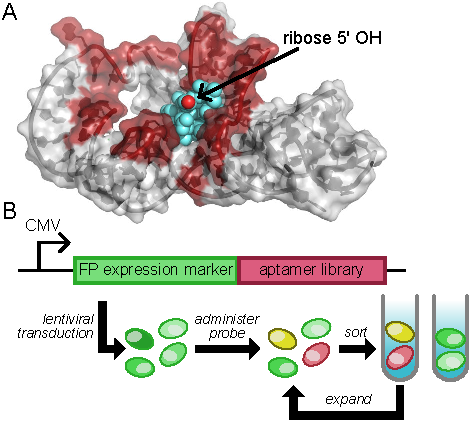
\includegraphics[width=\textwidth]{figures/aim2.pdf}

\end{centering}
\footnotesize
\caption{\label{figure:aim2}
A) Riboswitch sites for mutation will be targeted based on potential contact with the linker and fluorophore. PDB: 4FRN\cite{JohnsonJrB12cofactorsdirectly2012} B) RNA sequences will be screened for brightness relative to a fluorescent protein control.
}
\end{wrapfigure}
%%%%%%%%%%%%%%%%%%%%%%%%%%%%%%%%%%%%%%%%%%%%%%%%%%%%%%%%%%%%%%%%%%%%%%%%%%%%%%%%

First, a library will be designed that varies the environment surrounding the binding pocket of the cobalamin riboswitch (Fig. \ref{figure:aim2}A). Through the guidance of Robert Batey (see Batey support letter), sites will be chosen to retain binding of the cobalamin, yet maximize the distance between the quencher and the fluorophore upon binding\cite{JohnsonJrB12cofactorsdirectly2012}.
The Palmer lab is a leader in technologies for tool development in mammalian cells\cite{FiedlerDropletMicrofluidicFlow2017,DeanHighSpeedMultiparameterPhotophysical2015}.
This expertise will be leveraged for screening libraries of cobalamin riboswitches (Fig. \ref{figure:aim2}B). Libraries of transcripts will be transduced into mammalian cells, the probe of interest will be administered, and cells will be sorted via flow cytometry. Cells that show elevated brightness relative to a fluorescent protein expression control will be sorted.
In this way, libraries of up to one million members will be screened. Bright variants will be collected, cultured, and resubjected to sorting until only bright variants remain. Sequences will be evaluated through deep sequencing.

New sequences identified through this screen will undergo rigorous characterization of their biophysical and photophysical properties \textit{in vitro}. It will be important to characterize the extinction coefficient of each complex upon binding the RNA tag, as well as their quantum yields and photostability. The binding affinity for each probe-RNA combination will also be measured via isothermal titration calorimetry. Such a value is important because it informs the probe dosage that will be necessary for imaging (and lower probe dosages will contribute less fluorescence background).

Candidate probes that exhibit low background fluorescence, high signal induction, and high RNA affinity will be tested to determine the absolute level of turn-on fluorescence, and the minimum number of fluorophores that can be localized. To do this, beta actin mRNA will be tagged with one, two, or four repeats of the mutant riboswitch of interest in U2-OS cells through transient transfection. The cells will be imaged under conditions analogous to previous studies\cite{KatzMappingtranslationhotspots2016} using a TIRF microscope (see Equipment document). If puncta that appear to be single molecules are observed under these conditions, probe localization will be verified via fluorescence in situ hybridization (FISH) following cell fixation. If puncta are not visible in the initial TIRF images, cells will be treated with arsenite to induce the formation of stress granules (SGs) that also contain the protein G3BP1\cite{ZurlaCharacterizingmRNAInteractions2011,JainATPaseModulatedStressGranules2016,NellesProgrammableRNATracking2016}.
G3BP1 can be tagged with the Halo-tag, and subsequently labeled with an orthogonal fluorophore to evaluate colocalization. A check of direct mRNA location can then be carried out with FISH.
This is a technique that the Palmer lab has previously used successfully to test Riboglow probes\cite{BraselmannDevelopmentriboswitchbasedplatform2017}.

To quantify our ability to resolve single mRNA molecules, we will utilize single-molecule FISH (smFISH) imaging to correlate RNA count with Riboglow signal.\cite{TutucciimprovedMS2system2018} If the new Riboglow probes demonstrate single-molecule labeling in the beta actin model system, \comment{we will attempt to image transcipts of long, noncoding RNA (lncRNA) in the nucleus...}

% AMY Can propose to do this for a highly expressed transcript and a lower expressed transcript (could start by doing this for mRNA) but also do for a small nuclear RNA (involved in splicosome) or maybe better yet a long noncoding RNA....maybe look through some of John's papers and see if there are some that have distinct localizations....

% AMY Should address concern that tagging RNA perturbs RNA localization, dynamics and function and propose tests to evaluate this concern (localization can be assessed with live-fixed correlative smFISH experiments), function and dynamics are harder and may depend on the specific target.  Certainly the amount of RNA over time (so half life) can be assessed by Northern blotting (not perfect because population level as opposed to single cell, but still gets at the overall underlying concern).  This recent paper from Singer lab: https://www.ncbi.nlm.nih.gov/pubmed/29131164 may have some useful ideas of how to test perturbations and may even contain some ideas for target RNAs of interest.  This paper also has some intriguing ideas: https://www.ncbi.nlm.nih.gov/pubmed/29239719 (you could look at RNAs in cool, suprising locations)

\textbf{Summary and alternate approaches:}\\
To attain single-molecule resolution with Riboglow, the probes synthesized in Aim 1 will be screened with libraries of riboswitch mutants \textit{in cellulo}. Cells containing bright mutants will be sorted via FACS and analyzed. Library hits will be characterized \textit{in vitro}, and tested via established assays for single-molecule localization \textit{in cellulo}. Probes that are successful in our model systems will be used to image long, noncoding RNA under the supervision of Professor John Rinn. If single-molecule resolution is not observed in the library hits, additional riboswitches (over the four repeats already planned) will be added to concentrate fluorescent signal. Even if 24 repeats are required, the construct will still be less than half the size of the MS2 system.

%%%%%%%%%%%%%%%%%%%%%%%%%%%%%%%%%%%%%%%%%%%%%%%%%%%%%%%%%%%%%%%%%%%%%%%%%%%%%%%%
%Aim 3: Multicomponent imaging
%\begin{wrapfigure}[25]{l}{10cm}
\begin{wrapfigure}{L}{8cm}
%\vspace{-0.2in}
\begin{centering}
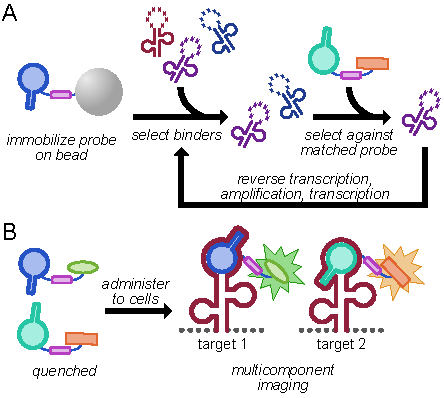
\includegraphics[width=\textwidth]{figures/aim3v2.pdf}
\end{centering}
\footnotesize
\caption{\label{figure:aim3}
A) SELEX will be used to screen for riboswitchs that bind each cobalamin in a mutually-exclusive manner. B) Mutually orthogonal cobalamin analogs will enable multicomponent RNA imaging. Signal turn-on will only be observed in the presence of the matched pair.
}
\end{wrapfigure}
%%%%%%%%%%%%%%%%%%%%%%%%%%%%%%%%%%%%%%%%%%%%%%%%%%%%%%%%%%%%%%%%%%%%%%%%%%%%%%%%

\textbf{\underline{Aim 3.} Develop mutually orthogonal Riboglow probes for multicomponent imaging.}\\
% TODO include precedent: \cite{HocineSinglemoleculeanalysisgene2013}
The ability to track multiple RNA transcripts simultaneously would enable study of the interactions of RNA as they move through the cell. \comment{Independent RNA transcripts are implicated to interact in X and Y ways.}
% AMY Could invoke the diagram of different RNAs and their processing/lifecycle.  Could be useful for looking at different mRNAs (dynamics of half life, processing) or for mRNAs and splicing RNAs or lncRNAs and their targets...
The modularity of the Riboglow platform is well suited to enable such an experiment. Probes will be distinguished through the use of different fluorophores, and different riboswitch sequences will be used to bind each structurally different probe in a mutually exclusive manner (Fig. \ref{figure:aim3}B).

Fortunately, screening for substrate selectivity is well-precedented in RNA engineering through systematic evolution of ligands by exponential enrichment (SELEX)\cite{MairalAptamersmoleculartools2008,ChoApplicationsAptamersSensors2009}.
In fact, \textit{de novo} riboswitches have already been developed for cobalamin and a few of its analogs via SELEX\cite{LorschvitroselectionRNA1994}. This important precedent shows that even small changes to the structure of the cobalamin can be distinguished by engineered RNA, and implies that no additional changes will need to be made to the cobalamin structure apart from those constructs already proposed above.

Importantly, for our selection experiments, we will not be starting from a completely randomized sequence of nucleic acids. It will be crucial to retain the original fold (and thus \textit{in cellulo} stability) of the native riboswitch. The design of the starting RNA libraries, and subsequent selection experiments will be carried out under the supervision of Professor Robert Batey (see Batey letter of support), an expert in SELEX and RNA engineering\cite{TrauschChapterThreeDesign2015}.
The selection will be carried out as shown in Figure \ref{figure:aim3}A. Briefly, cobalamin probe of interest will be immobilized on a bead via the same linker that will be used in the final construct. The synthetic library of riboswitches will be incubated with the beads, and unbound sequences will be rinsed away. In a second rinsing step, the probe (or probes) intended to be orthogonal to the construct under selection will be incubated with the beads to wash away any riboswitches that do not bind selectively. \comment{Is this kind of negative screen known?}
% AMY This is a nice (and recent) paper from the Batey lab: https://www.nature.com/articles/nchembio.2278.pdf Details multiple rounds of selection under increasingly stringent conditions (something you should probably propose) as well as counter selections.  In fact the paper does a nice job of detailing some selection details and you may want to include information like this in your proposal.
Riboswitches that bind selectively will be collected off the beads and amplified (via reverse transcription, PCR amplification, and transcription) to undergo another round of selection. Riboswitches will be deep sequenced to identify library convergence and optimal clones. This process will be repeated for each probe of interest, with negative screens against each other probe that is intended for multiplexed use.
% TODO make a point here about how unnatural ligand architectures will help reduce off-target fluorescence.

Once mutually-selective Riboglow probes are identified, they will be tested in mammalian cells...
% AMY But before you do proof of concept - simultaneous detection of 2 RNAs in live cell - you need to do the same level of characterization of these selective aptamer-probe pairs that you did in aim 2, in vitro and cellular characterization.
\comment{Maybe look at two differently localized RNAs that both migrate to SGs upon arsenite addition?}
% AMY For simultaneous detection of RNA, you want to propose a proof of concept experiment where it needs to be done in live cells, so something that requires an analysis of dynamics (of association, of localization, of half life, etc).  You could either look at differential sequestration of RNAs to ribonucleoprotein complexes like stress granules (https://www.ncbi.nlm.nih.gov/pubmed/29483269 may have some ideas).  Also the stress granule transcriptome: https://scholar.google.com/scholar_lookup?author=A+Khong&title=The+stress+granule+transcriptome+reveals+principles+of+mRNA+accumulation+in+stress+granules&publication_year=2017&journal=Mol+Cell&volume=68&pages=808-820.e5

\textbf{Summary and alternate approaches:}

%%% Local Variables: ***
%%% mode: latex ***
%%% TeX-master: "Research_and_SA.tex" ***
%%% End: ***
